\documentclass{article}
\usepackage[backend=biber,natbib=true,style=alphabetic,maxbibnames=50]{biblatex}
\addbibresource{/home/nqbh/reference/bib.bib}
\usepackage[utf8]{vietnam}
\usepackage{tocloft}
\renewcommand{\cftsecleader}{\cftdotfill{\cftdotsep}}
\usepackage[colorlinks=true,linkcolor=blue,urlcolor=red,citecolor=magenta]{hyperref}
\usepackage{amsmath,amssymb,amsthm,float,graphicx,mathtools,tikz}
\usetikzlibrary{angles,calc,intersections,matrix,patterns,quotes,shadings}
\allowdisplaybreaks
\newtheorem{assumption}{Assumption}
\newtheorem{baitoan}{}
\newtheorem{cauhoi}{Câu hỏi}
\newtheorem{conjecture}{Conjecture}
\newtheorem{corollary}{Corollary}
\newtheorem{dangtoan}{Dạng toán}
\newtheorem{definition}{Definition}
\newtheorem{dinhly}{Định lý}
\newtheorem{dinhnghia}{Định nghĩa}
\newtheorem{example}{Example}
\newtheorem{ghichu}{Ghi chú}
\newtheorem{hequa}{Hệ quả}
\newtheorem{hypothesis}{Hypothesis}
\newtheorem{lemma}{Lemma}
\newtheorem{luuy}{Lưu ý}
\newtheorem{nhanxet}{Nhận xét}
\newtheorem{notation}{Notation}
\newtheorem{note}{Note}
\newtheorem{principle}{Principle}
\newtheorem{problem}{Problem}
\newtheorem{proposition}{Proposition}
\newtheorem{question}{Question}
\newtheorem{remark}{Remark}
\newtheorem{theorem}{Theorem}
\newtheorem{vidu}{Ví dụ}
\usepackage[left=1cm,right=1cm,top=5mm,bottom=5mm,footskip=4mm]{geometry}
\def\labelitemii{$\circ$}
\DeclareRobustCommand{\divby}{%
	\mathrel{\vbox{\baselineskip.65ex\lineskiplimit0pt\hbox{.}\hbox{.}\hbox{.}}}%
}

\title{Problem: 1st-Order Function -- Bài Tập: Hàm Số Bậc Nhất $y = ax + b$, $a\ne0$}
\author{Nguyễn Quản Bá Hồng\footnote{Independent Researcher, Ben Tre City, Vietnam\\e-mail: \texttt{nguyenquanbahong@gmail.com}; website: \url{https://nqbh.github.io}.}}
\date{\today}

\begin{document}
\maketitle
\tableofcontents

%------------------------------------------------------------------------------%

\section{Khái Niệm Hàm Số}

\begin{baitoan}[\cite{Binh_boi_duong_Toan_9_tap_1}, H3, p. 49]
	Tìm $a\in\mathbb{R}$ để điểm $A(-1,3)$ thuộc đồ thị hàm số $y = ax^2$.
\end{baitoan}

\begin{baitoan}[\cite{Binh_boi_duong_Toan_9_tap_1}, H4, p. 49]
	Cho hàm số $y = f(x)$ xác định trên $\mathbb{R}$. (a) Nếu giá trị của biến $x$ tăng lên mà giá trị tương ứng $f(x)$ cũng tăng lên thì hàm số $y = f(x)$ được gọi là $\ldots$ trên $\mathbb{R}$. (b) Nếu giá trị của biến $x$ tăng lên mà giá trị tương ứng $f(x)$ $\ldots$ thì hàm số $y = f(x)$ được gọi là nghịch biến trên $\mathbb{R}$.
\end{baitoan}

\begin{baitoan}[\cite{Binh_boi_duong_Toan_9_tap_1}, H5, p. 49]
	(a) Tìm {\rm TXĐ} của hàm số $y = \dfrac{1}{\sqrt{2 - x}}$. (b) Tìm {\rm TXĐ} của hàm số $y = \dfrac{2x + 1}{x^2 - 3x + 2}$.
\end{baitoan}

\begin{baitoan}[\cite{Binh_boi_duong_Toan_9_tap_1}, VD1, p. 49]
	Ở bưu điện, giá tiền cước gửi thư trong nước được niêm yết như sau (chưa tính {\rm VAT}):
	\begin{table}[H]
		\centering
		\begin{tabular}{|l|c|}
			\hline
			Nấc khối lượng (g) & Mức cước (đồng) \\
			\hline
			Đến 20 g & 2000 \\
			\hline
			Trên 20 g đến 100 g & 3000 \\
			\hline
			Trên 100 g đến 250 g & 4500 \\
			\hline
			Mỗi 250 g tiếp theo đến 2000 g & 2000 \\
			\hline
		\end{tabular}
	\end{table}
	\noindent Nếu gọi khối lượng lá thư là $x$ {\rm g}, số tiền cước phải trả là $y$ đồng. (a) $y$ có là hàm số của $x$ không? Vì sao? (b) Tìm {\rm TXĐ} của hàm số $y$. (c) 1 lá thư nặng {\rm300 g} cần phải trả tiền cước là bao nhiêu? (d) Hỏi $x$ có là hàm số của $y$ không? Vì sao?
\end{baitoan}

\begin{baitoan}[\cite{Binh_boi_duong_Toan_9_tap_1}, VD2, p. 50]
	1 ôtô có bình chứa xăng đựng được {\rm40 L} xăng. Cứ chạy {\rm100 km} thì ôtô tiêu thụ hết {\rm8 L} xăng. (a) Khi ôtô chạy $x$ {\rm km} thì số {\rm L} xăng $y$ tiêu thụ là bao nhiêu? (b) Hỏi $y$ có là 1 hàm số của $x$ không? (c) Hỏi $x$ có là 1 hàm số của $y$ không? (d) Khi ôtô chạy được {\rm200 km} thì số {\rm L} xăng còn lại trong bình là bao nhiêu nếu lúc đầu bình đầy?
\end{baitoan}

\begin{baitoan}[\cite{Binh_boi_duong_Toan_9_tap_1}, VD3, p. 51]
	Vẽ trên mặt phẳng tọa độ $Oxy$ các điểm $A(0,5),B(4,5),C(4,0),M(x,0$ với $x > 4$, $N(0,2)$. (a) Tính diện tích S của tứ giác $OABC$. (b) Tính diện tích P của $\Delta BMN$ theo $x$. Chứng minh P là hàm số của $x$. (c) Tìm {\rm TXĐ} của $P$. Hàm số P đồng biến hay nghịch biến trên {\rm TXĐ} của nó? (d) Với giá trị nào của $x$ thì $S = P$?
\end{baitoan}

\begin{baitoan}[\cite{Binh_boi_duong_Toan_9_tap_1}, VD4, p. 51]
	Cho hình chữ nhật ABCD với $AB = 36,BC = 15$. Trên cạnh AB lấy điểm M. Gọi $AM = x$, $0 < x < 36$. Qua M kẻ $MN\parallel BD$ với $N\in AD$. Qua M kẻ $MP\parallel AC$ với $P\in BC$. (a) Chứng minh độ dài $MN,MP$ là 2 hàm số của $x$. (b) Trên cạnh CD lấy điểm Q sao cho $DQ = 36 - x$. Chứng minh chu vi tứ giác MNQP là 1 hàm hằng.
\end{baitoan}

\begin{baitoan}[\cite{Binh_boi_duong_Toan_9_tap_1}, VD5, p. 52]
	Đồ thị hàm số $y = f(x)$ trên mặt phẳng tọa độ: $A(-3,3),B(-1,-3),C(2,-3),D(4,0)$.
	\begin{center}
		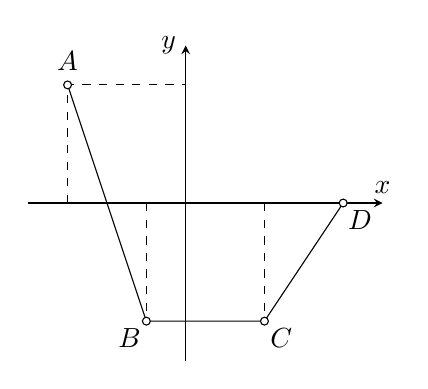
\begin{tikzpicture}[>=stealth]
			\draw[->](-2,0)--(5/2,0) node[above]{$x$};
			\draw[->](0,-2)--(0,2) node[left]{$y$};
			\draw[dashed](-3/2,0)--(-3/2,3/2)--(0,3/2) (-1/2,0)--(-1/2,-3/2) (1,0)--(1,-3/2);
			\path
			(0,0) coordinate (O)
			(-3/2,3/2) coordinate (A)
			(-1/2,-3/2) coordinate (B)
			(1,-3/2) coordinate (C)
			(2,0) coordinate (D);
			\draw (A)--(B)--(C)--(D);
			\foreach \x/\g in {A/90,B/-135,C/-45,D/-45} \draw[fill=white] (\x) circle (.05) + (\g:.3) node{$\x$};
		\end{tikzpicture}
	\end{center}
	\noindent(a) Tìm {\rm TXĐ} của hàm số $y$. (b) Tính $f(-3),f(-1),f(1),f(2),f(3),f(4)$. (c) Hàm số $y = f(x)$ đồng biến \& nghịch biến trong khoảng nào? (d) {\rm Đ{\tt/}S?} Khi xét $x_1 = 2$, $f(x_1) = f(2) = -3$, $x_2 = -3$, $f(x_2) = f(-3) = 3$, ta thấy $x_2 < x_1$, $f(x_2) > f(x_1)$ nên hàm số nghịch biến trong khoảng $[-3,2]$.
\end{baitoan}

\begin{baitoan}[\cite{Binh_boi_duong_Toan_9_tap_1}, 6.1., p. 53]
	Bảng sau ghi các giá trị tương ứng của 2 đại lượng $x,y$ phụ thuộc nhau.
	\begin{table}[H]
		\centering
		\begin{tabular}{|c|c|c|c|c|c|c|c|c|c|}
			\hline
			$x$ & 1 & 2 & 3 & 4 & 5 & 1 & 6 & 7 & 8 \\
			\hline
			$y$ & 0 & 2 & -1 & 5 & 4 & -4 & 3 & -2 & -6 \\
			\hline
		\end{tabular}
	\end{table}
	\noindent(a) $y$ có là hàm số của $x$ không? (b) $x$ có là hàm số của $y$ không? (c) Trường hợp là hàm số, nêu {\rm TXĐ}.
\end{baitoan}

\begin{baitoan}[\cite{Binh_boi_duong_Toan_9_tap_1}, 6.2., p. 53]
	Cho hàm số $y = f(x) = 3x^2 + 1$. (a) Tính $f(-1),f(0),f(1)$. (b) Tìm $x$ để $f(x) = 4$. (c) Trong 3 điểm $A(0,1),B(2,3),C(3,4)$, điểm nào không thuộc đồ thị hàm số đã cho?
\end{baitoan}

\begin{baitoan}[\cite{Binh_boi_duong_Toan_9_tap_1}, 6.3., p. 53]
	Bảng giá bán lẻ điện cho các hộ gia đình (chưa tính {\rm VAT}) (theo QĐ số 2256{\tt/}QĐ-BCT 12.3.2015 của Bộ Công thương):
	\begin{table}[H]
		\centering
		\begin{tabular}{|l|c|}
			\hline
			Mức độ sử dụng của mỗi hộ trong tháng & Giá bán điện (đồng{\tt/}kwh) \\
			\hline
			Bậc 1: cho kwh từ 0--50 & 1484 \\
			\hline
			Bậc 2: cho kwh từ 51--100 & 1533 \\
			\hline
			Bậc 3: cho kwh từ 101--200 & 1786 \\
			\hline
			Bậc 4: cho kwh từ 201--300 & 2242 \\
			\hline
			Bậc 5: cho kwh từ 301--400 & 2503 \\
			\hline
			Bậc 6: cho kwh từ 401 trở lên & 2587 \\
			\hline
		\end{tabular}
	\end{table}
	\noindent Gọi số điện sử dụng của hộ gia đình là $x$ {\rm kwh}, số tiền phải trả là $y$ đồng. (a) $y$ có phải là hàm số của $x$ không? (b) Nếu dùng hết $310$ {\rm kwh} điện thì phải trả bao nhiêu tiền?
\end{baitoan}

\begin{baitoan}[\cite{Binh_boi_duong_Toan_9_tap_1}, 6.4., p. 53]
	Chứng minh: (a) Hàm số $y = 2x + 3$ đồng biến trên $\mathbb{R}$. (b) Hàm số $y = -2x + 7$ nghịch biến trên $\mathbb{R}$.
\end{baitoan}

\begin{baitoan}[\cite{Binh_boi_duong_Toan_9_tap_1}, 6.5., p. 53]
	Cho $\Delta ABC$ đều có độ dài cạnh bằng $a$. Lấy $M\in AB$ sao cho $AM = x$ với $0 < x < a$. Vẽ hình chữ nhật MNPQ với $N\in AC$, $P,Q\in BC$. (a) Chứng minh diện tích hình chữ nhật MNPQ là hàm số của $x$. (b) Xác định $x$ để diện tích hình chữ nhật MNPQ lớn nhất.
\end{baitoan}

\begin{baitoan}[\cite{Binh_boi_duong_Toan_9_tap_1},  p. 53, Công thức Lorentz cho số cân nặng lý tưởng tương ứng với chiều cao]
	Cách đây hơn 1 thế kỷ, nhà khoa học người Hà Lan Hendrick Lorentz (1853--1928) đưa ra công thức tính số cân nặng lý tưởng của con người theo chiều cao:
	\begin{align*}
		\boxed{M = T - 100 - \dfrac{T - 150}{N}}
	\end{align*}
	trong đó $M$: số cân nặng {\rm kg}, $T$: chiều cao {\rm cm}, $N = 4$ với nam giới \& $N = 2$ với nữ giới. (a) Kiểm chứng công thức với cân nặng \& chiều cao của bản thân. (b) Viết công thức tính số cân nặng lý  tưởng của nam giới (ký hiệu là $P_1$) \& số cân nặng lý tưởng của nữ giới (ký hiệu là $P_2$) theo chiều cao. (c) Vẽ đồ thị hàm $M$ theo $T$. (d) $P_1,P_2$ có phải là hàm số của $T$ không? (c) Với $T$ bằng bao nhiêu thì $P_1 = P_2$?
\end{baitoan}

%------------------------------------------------------------------------------%

\section{1st-Order Function \& Its Graph -- Hàm Số Bậc Nhất \& Đồ Thị Của Nó}

\begin{baitoan}[\cite{Binh_boi_duong_Toan_9_tap_1}, H1, p. 55]
	$y$ là hàm số bậc nhất của $x\Leftrightarrow$: {\sf A.} $y = ax + b$, $a,b\in\mathbb{R}$. {\sf B.} $y = ax + b$, $a,b\in\mathbb{R}$, $ab\ne0$. {\sf C.} $y = ax + b$, $a,b\in\mathbb{R}$, $b\ne0$. {\sf D.} $y = ax + b$, $a,b\in\mathbb{R}$, $a\ne0$.
\end{baitoan}

\begin{baitoan}[\cite{Binh_boi_duong_Toan_9_tap_1}, H2, p. 55]
	Phân loại hàm số: (a) $y = \sqrt{2}(x - 1)$. (b) $y = \sqrt{2x} - 1$. (c) $y = \dfrac{x^2}{x} + 4$. (d) $y = \dfrac{2}{x} + 1$.
\end{baitoan}

\begin{baitoan}[\cite{Binh_boi_duong_Toan_9_tap_1}, H3, p. 56]
	Cho hàm số $y = (m + 1)x + 3m$. Khi đó: {\sf A.} $y$ là hàm số bậc nhất của biến $x$. {\sf B.} $y$ là hàm số bậc nhất của biến $m$. {\sf C.} $y$ là hàm số bậc nhất. {\sf D.} Với $m\ne-1$, $y$ là hàm số bậc nhất của biến $x$.
\end{baitoan}

\begin{baitoan}[\cite{Binh_boi_duong_Toan_9_tap_1}, H4, p. 56]
	Tìm điều kiện của $m$ để hàm số $y = (3m - 6)x + 8$ đồng biến trên $\mathbb{R}$.
\end{baitoan}

\begin{baitoan}[\cite{Binh_boi_duong_Toan_9_tap_1}, H5, p. 56]
	Vẽ đồ thị hàm số $y = -\dfrac{1}{2}x + 1$.
\end{baitoan}

\begin{baitoan}[\cite{Binh_boi_duong_Toan_9_tap_1}, VD1, p. 56]
	Với các giá trị nào của $m$ thì mỗi hàm số sau là hàm số bậc nhất? (a) $y = \sqrt{4 - m}(x - 1)$. (b) $y = \dfrac{m + 2}{m - 2}x + 3.5 + x$.
\end{baitoan}

\begin{baitoan}[\cite{Binh_boi_duong_Toan_9_tap_1}, VD2, p. 57]
	1 hình chữ nhật có 2 kích thước là {\rm10 cm, 15 cm}. Bớt mỗi kích thước của hình chữ nhật đi $x$ {\rm cm} với $0 < x < 10$. Gọi chu vi của hình chữ nhật mới là $y$ {\rm cm}. (a) Lập công thức tính chu vi $y$ của hình chữ nhật mới theo $x$. (b) Chứng minh $y$ là hàm số bậc nhất của $x$ \& vẽ đồ thị hàm số đó.
\end{baitoan}

\begin{baitoan}[\cite{Binh_boi_duong_Toan_9_tap_1}, VD3, p. 57]
	(a) Vẽ đồ thị 2 hàm số $y = x - 2$ \& $y = -x - 1$ trên cùng 1 mặt phẳng tọa độ. (a) 2 đường thẳng $y = -x - 1$ \& $y = x - 2$ cắt nhau tại C \& cắt trục $Ox$ theo thứ tự $A,B$. Tìm tọa độ của 3 điểm $A,B,C$. (c) Chứng minh $\Delta ABC$ vuông cân. (d) Tính chu vi \& diện tích $\Delta ABC$.
\end{baitoan}

\begin{baitoan}[\cite{Binh_boi_duong_Toan_9_tap_1}, VD4, p. 58]
	Cho hàm số $y = (2m + 1)x + m - 1$ với $m\ne-\dfrac{1}{2}$. (a) Xác định $m$ trong mỗi trường hợp: (i) Đồ thị hàm số đi qua $M(1,1)$. (ii) Đồ thị cắt trục tung, trục hoành lần lượt tại $A,B$ sao cho $\Delta OAB$ cân. (iii) Đồ thị cắt trục tung, trục hoành lần lượt tại $A,B$ sao cho $\Delta OAB$ có diện tích bằng $\dfrac{1}{2}$. (b) Tìm giá trị nguyên của $m$ để đồ thị cắt trục hoành tại điểm có hoành độ là số nguyên. (c) Tìm các điểm cố định mà đồ thị hàm số luôn đi qua với mọi giá trị của $m$.
\end{baitoan}

\begin{baitoan}[\cite{Binh_boi_duong_Toan_9_tap_1}, 7.1., p. 60]
	Cho 3 hàm số $y = 2x + 1$, $y = 4x$, $y = -2x + 5$ theo thứ tự có đồ thị là 3 đường thẳng $(d_1),(d_2),(d_3)$. (a) Trong 3 hàm số này, hàm số nào đồng biến, hàm số nào nghịch biến? (b) Vẽ $(d_1),(d_2),(d_3)$ trên cùng 1 mặt phẳng tọa độ. (c) Trong 4 điểm $A(1,3),B(0,4),C(-1,-4),D(-2,9)$ có điểm nào nằm trên $(d_1)$ hoặc $(d_2)$ hoặc $(d_3)$ không?
\end{baitoan}

\begin{baitoan}[\cite{Binh_boi_duong_Toan_9_tap_1}, 7.2., p. 61]
	Lập công thức biểu thị $y$ theo $x$. Cho biết công thức nào là hàm số bậc nhất (chỉ rõ $a,b$). (a) Diện tích tam giác $y$ $\rm cm^2$ có đáy là $x$ {\rm cm} \& chiều cao tương ứng là {\rm6 cm}. (b) Chu vi hình thoi $y$ {\rm cm} với cạnh là $x$ {\rm cm}. (c) Chu vi đường tròn $y$ {\rm cm} với bán kính là $x$ {\rm cm}. (d) Diện tích hình tròn $y$ $\rm cm^2$ với bán kính là $x$ {\rm cm}.
\end{baitoan}

\begin{baitoan}[\cite{Binh_boi_duong_Toan_9_tap_1}, 7.3., p. 61]
	Trong mặt phẳng tọa độ $Oxy$ cho 3 điểm $A(2,-1),B(-1,-7),C(3,1)$. (a) Viết phương trình đường thẳng BC. (b) Chứng minh 3 điểm $A,B,C$ thẳng hàng.
\end{baitoan}

\begin{baitoan}[\cite{Binh_boi_duong_Toan_9_tap_1}, 7.4., p. 61]
	Cho hàm số $y = (m - 2)x + 3$. (a) Với giá trị nào của $m$ thì hàm số đồng biến, nghịch biến, hàm hằng? (b) Xác định giá trị của $m$ để đồ thị hàm số đi qua điểm $A(1,4)$. (c) Vẽ đồ thị hàm số ứng với giá trị của $m$ tìm được ở (b).
\end{baitoan}

\begin{baitoan}[\cite{Binh_boi_duong_Toan_9_tap_1}, 7.5., p. 61]
	Cho 6 đường thẳng chứa 4 cạnh \& 2 đường chéo của 1 hình chữ nhật có tâm trùng với gốc tọa độ. Tìm số đường thẳng là đồ thị của 1 hàm số bậc nhất?
\end{baitoan}

\begin{baitoan}[\cite{Binh_boi_duong_Toan_9_tap_1}, 7.6., p. 61]
	Lập phương trình đường thẳng đi qua 2 điểm $A,B$ với: (a) $A(2,3),B(2,5)$. (b) $A(1,4),B(-5,4)$. (c) $A(2,2),B(-4,3)$. Từ đó đưa ra công thức tổng quát phương trình đường thẳng đi qua $A(x_1,y_1)$ \& $B(x_2,y_2)$.
\end{baitoan}

\begin{baitoan}[\cite{Binh_boi_duong_Toan_9_tap_1}, 7.7., p. 61]
	Cho 3 đường thẳng $(d_1):y = 1 - x$, $(d_2):x - y = 3$, $(d_3):(m + 1)x + (m - 1)y = 1 + 2m$. (a) Xác định $m$ để 3 đường thẳng cùng đi qua 1 điểm. (b) Chứng minh khi $m$ thay đổi, đường thẳng $(d_3)$ luông đi qua 1 điểm cố định.
\end{baitoan}

\begin{baitoan}[\cite{Binh_boi_duong_Toan_9_tap_1}, 7.8., p. 61]
	Cho hàm số $y = (m^2 + m + 1)x + 6$ có đồ thị $(d)$. (a) Chứng minh: $\forall m\in\mathbb{R}$, $y$ luôn là hàm số bậc nhất đồng biến. (b) Tìm $m$ để $(d)$ cắt $Ox$ tại A, cắt $Oy$ tại B sao cho: (i) Diện tích $\Delta AOB$ bằng $4$. (ii) Diện tích $\Delta AOB$ lớn nhất.
\end{baitoan}

\begin{baitoan}[\cite{Binh_boi_duong_Toan_9_tap_1}, p. 62, Mối quan hệ giữa độ F \& độ C]
	Độ Fahrenheit (độ {\rm F} hay ${}^\circ${\rm F}) là thang nhiệt được đặt theo tên nhà Vật lý người Đức Gabriel Fahrenheit (1686--1736) -- người đã đề xuất ra nó năm 1724. Theo đó, nước đóng bằng ở $32^\circ${\rm F} \& sôi ở $212^\circ${\rm F} (2 trạng thái này chênh lệch $180^\circ${\rm F}). Độ Celsius (độ {\rm C} hay ${}^\circ${\rm C}) là thang nhiệt được đặt theo tên nhà thiên văn học người Thụy Điển Anders Celsius (1701--1744) -- người đầu tiên đề nghị hệ thống đo nhiệt độ {\rm C} năm 1742 \& đến năm 1750, độ {\rm C} còn được gọi là độ bách phân. Theo đó, nước đóng băng ở $0^\circ${\rm C} \& sôi ở $100^\circ${\rm C}. Do đó, mỗi độ thuộc thang đo Celcius bằng $\dfrac{212 - 32}{100 - 0} = \dfrac{180}{100} = \dfrac{9}{5}$ độ thuộc thang đo Fahrenheit. Ngày nay, đa số các nước sử dụng thang nhiệt độ là độ {\rm C}, tuy nhiên 1 số nước, e.g., Mỹ, vẫn sử dụng nhiệt kế chia mức độ nhiệt độ theo độ {\rm F}. Mối quan hệ giữa số đo độ {\rm F}, ký hiệu là $T_{\rm F}$, \& số đo độ {\rm C}, ký hiệu là $T_{\rm C}$: $T_{\rm F} = 1.8TT_{\rm C} + 32$. (a) $T_{\rm F},T_{\rm C}$ có là hàm số bậc nhất có nhau không. (b) Xét tính đồng biến, nghịch biến của 2 hàm số này.
\end{baitoan}

\begin{baitoan}[\cite{Binh_boi_duong_Toan_9_tap_1}, VD1, p. 63]
	Xét sự biến thiên \& vẽ đồ thị hàm số $y = |2x + 3|$.
\end{baitoan}

\begin{baitoan}[\cite{Binh_boi_duong_Toan_9_tap_1}, VD2, p. 63]
	Cho hàm số $y = |x - 1| + |x - 5|$. (a) Vẽ đồ thị hàm số. (b) Xác định {\rm GTNN} của hàm số.
\end{baitoan}

\begin{baitoan}[\cite{Binh_boi_duong_Toan_9_tap_1}, p. 64]
	Xét sự biến thiên \& vẽ đồ thị hàm số: (a) $y = |-3x + 1|$. (b) $y = |x + 1| + |2x - 3|$.
\end{baitoan}

%------------------------------------------------------------------------------%

\section{Đường Thẳng Song Song \& Đường Thẳng Cắt Nhau. Hệ Số Góc Của Đường Thẳng $y = ax + b$, $a\ne0$}

%------------------------------------------------------------------------------%

\section{Miscellaneous}

%------------------------------------------------------------------------------%

\printbibliography[heading=bibintoc]
	
\end{document}